\documentclass[a4paper,12pt, titlepage]{report} % размер бумаги устанавливаем А4, шрифт 12пунктов
\usepackage[T2A]{fontenc}
\usepackage[utf8]{inputenc} % включаем свою кодировку: koi8-r или utf8 в UNIX, cp1251 в Windows
\usepackage[english,russian]{babel} % используем русский и английский языки с переносами
\usepackage{amssymb,amsfonts,amsmath,mathtext,cite,enumerate,float} % подключаем нужные пакеты расширений
\usepackage[dvips]{graphicx} % хотим вставлять в диплом рисунки?
\usepackage{graphicx}
\usepackage{grffile}
\graphicspath{{figure/}} % путь к рисункам

\makeatletter
\renewcommand{\@biblabel}[1]{#1.} % Заменяем библиографию с квадратных скобок на точку:
\makeatother

\usepackage{geometry} % Меняем поля страницы
\geometry{left=2.5cm} % левое поле
\geometry{right=1.5cm} % правое поле
\geometry{top=2cm} % верхнее поле
\geometry{bottom=2cm} % нижнее поле

\renewcommand{\theenumi}{\arabic{enumi}.} % Меняем везде перечисления на цифра.цифра
\renewcommand{\labelenumi}{\arabic{enumi}.} % Меняем везде перечисления на цифра.цифра
\renewcommand{\theenumii}{.\arabic{enumii}.} % Меняем везде перечисления на цифра.цифра
\renewcommand{\labelenumii}{\arabic{enumi}.\arabic{enumii}.} % Меняем везде перечисления на цифра.цифра
\renewcommand{\theenumiii}{.\arabic{enumiii}.} % Меняем везде перечисления на цифра.цифра
\renewcommand{\labelenumiii}{\arabic{enumi}.\arabic{enumii}.\arabic{enumiii}.} % Меняем везде перечисления на цифра.цифра

%\usepackage{fontspec} % Подключение специальных шрифтов
%\setmainfont[Mapping=tex-text]{Times New Roman}  % Times New Roman

\usepackage[onehalfspacing]{setspace} %"умное" расстояние между строк - установить 1.5 интервала от нормального, эквивалентно

\usepackage{indentfirst} % Отделять первую строку раздела абзацным отступом тоже

\newcommand{\empline}{\mbox{}\newline}
\newcommand{\likechapterheading}[1]{
	\begin{center}
		\textbf{\MakeUppercase{#1}}
	\end{center}
}

\usepackage{titlesec}
\titleformat{\chapter}[display]{\filcenter}{\MakeUppercase{\chaptertitlename} \thechapter}{8pt}{\bfseries \MakeUppercase}{}\titleformat{\section}{\normalsize\bfseries}   {\thesection.}{1em}{}\titleformat{\subsection}{\normalsize\bfseries}{\thesubsection.}{1em}{}% Настройка вертикальных и горизонтальных отступов
\titlespacing*{\chapter}{0pt}{-30pt}{8pt}
\titlespacing*{\section}{\parindent}{*4}{*1}
\titlespacing*{\subsection}{\parindent}{*4}{*1}
\titlespacing*{\subsubsection}{\parindent}{*4}{*1}

\makeatletter
\renewcommand{\@dotsep}{2}\newcommand{\l@likechapter}[2]{{\bfseries\@dottedtocline{1}{0pt}{0pt}{#1}{#2} }} \makeatother \newcommand{\likechapter}[1]{
\newpage \likechapterheading{#1}

\addcontentsline{toc}{likechapter}{\MakeUppercase{#1}}}

\usepackage{tocloft}
\renewcommand\contentsname{Оглавление}
\renewcommand{\cfttoctitlefont}{\hspace{0.38\textwidth}\bfseries\MakeUppercase } % Оформление надписи Оглавление
\renewcommand{\cftbeforetoctitleskip}{-1em}
%\renewcommand{\cftaftertoctitle}{\mbox{}\hfill \\ \mbox{}\hfill{\footnotesize Стр.}\vspace{-2.5em}} % Добавим надпись стр.
\renewcommand{\cftchapleader}{\cftdotfill{\cftdotsep}} % Отточия после глав
\renewcommand{\cftchapaftersnum}{.} % Точка после номера главы
\renewcommand{\cftsecaftersnum}{.} % Точка после номера параграфа

%\renewcommand{\cftchapfont}{\normalsize\bfseries \MakeUppercase{\chaptername} } % Оформления надписи Глава
\renewcommand{\cftsecfont}{\hspace{15pt}} % Сдвиг названия секции от левого края
\renewcommand{\cftsubsecfont}{\hspace{1pt}}
\renewcommand{\cftbeforechapskip}{1em}
\renewcommand{\cftparskip}{-1mm}
\renewcommand{\cftdotsep}{1} \setcounter{tocdepth}{1} % Задать глубину оглавления — до subsection включительно
\renewcommand{\cftdotsep}{2} \setcounter{tocdepth}{2} % Задать глубину оглавления — до subsubsection включительно

% Оформление подписи к рисункам и таблицам
\usepackage[font=small, tableposition=top]{caption}
\usepackage{subcaption}
\DeclareCaptionLabelFormat{gostfigure}{Рисунок #2}
\DeclareCaptionLabelFormat{gosttable}{Таблица #2}
\DeclareCaptionLabelSeparator{gost}{. }
\captionsetup{labelsep=gost}
\captionsetup[figure]{labelformat=gostfigure}
\captionsetup[table]{labelformat=gosttable}
\renewcommand{\thesubfigure}{\asbuk{subfigure}}

\usepackage[title,titletoc]{appendix}
\titleformat{\paragraph}[display]{\filcenter}{\MakeUppercase{\chaptertitlename} \thechapter}{8pt}{\bfseries}{}
\titlespacing*{\paragraph}{0pt}{-30pt}{8pt}
\newcommand{\append}[1]{\clearpage
\stepcounter{chapter}
\paragraph{\MakeUppercase{#1}}
\empline     \addcontentsline{toc}{likechapter}{\MakeUppercase{\chaptertitlename~\Asbuk{chapter}.\;#1}}}

\bibliographystyle{utf8gost705u}
%\usepackage[nottoc,notlot,notlof]{tocbibind}
\usepackage[square,numbers,sort&compress]{natbib}
\renewcommand{\bibnumfmt}[1]{#1.\hfill} % нумерация источников в самом списке — через точку
\renewcommand{\bibsection}{\likechapter{Литература}} % заголовок специального раздела
\setlength{\bibsep}{0pt}

\usepackage{listings}
\usepackage{color}
\usepackage{xcolor}

\lstdefinestyle{customc}{
  belowcaptionskip=1\baselineskip,
  breaklines=true,
  frame=L,
  xleftmargin=\parindent,
  showstringspaces=false,
  basicstyle=\footnotesize\ttfamily,
  keywordstyle=\bfseries\color{green!40!black},
  commentstyle=\itshape\color{purple!40!black},
  identifierstyle=\color{blue},
  stringstyle=\color{orange},
  numbers=left,               % где поставить нумерацию строк (слева\справа)
  numberstyle=\tiny  
}

\lstdefinestyle{customasm}{
  belowcaptionskip=1\baselineskip,
  frame=L,
  xleftmargin=\parindent,
  language=[x86masm]Assembler,
  basicstyle=\footnotesize\ttfamily,
  commentstyle=\itshape\color{purple!40!black},
}

\lstset{escapechar=@,style=customc}

%\usepackage[koi8-r]{inputenc}%включаем свою кодировку: koi8-r или utf8 в UNIX, cp1251 в Windows

\usepackage{enumitem}
\makeatletter
\AddEnumerateCounter{\asbuk}{\@asbuk}{м)}
\makeatother
\setlist{nolistsep}
\renewcommand{\labelitemi}{-}
\renewcommand{\labelenumi}{\asbuk{enumi})}
\renewcommand{\labelenumii}{\arabic{enumii})}

\usepackage{amsthm}
\theoremstyle{plain}
\newtheorem{thm}{Theorem}[section]
%\newtheorem{thm}{Theorem}[subsection]
%\newtheorem{defn}[thm]{Definition}
\newtheorem{St}{Утверждение}
\newtheorem{Th}{Теорема}
\newtheorem{Cor}{Следствие}
\newtheorem{Lm}{Лемма}

\usepackage{hyperref} 
\begin{document}

	\singlespacing % Одинарный междустрочный интервал
	\begin{titlepage}
	\newpage
	\begin{center}
		
\includegraphics[width=0.8cm]{logo_unn_crop.eps} \\*
		МИНИСТЕРСТВО НАУКИ И ВЫСШЕГО ОБРАЗОВАНИЯ\\
		РОССИЙСКОЙ ФЕДЕРАЦИИ
		\\*
		%\vspace{1cm}
		Федеральное государственное автономное образовательное учреждение\\* высшего образования \\*
		\textbf{<<Национальный исследовательский \\* Нижегородский государственный университет им. Н.И. Лобачевского>>\\* (ННГУ)\\*}\\*
		%\hrulefill
		\vspace{2em}
		\textbf{Институт информационных технологий, математики и механики}\\*
		\textbf{Направление подготовки: <<Фундаментальная информатика и информационные технологии>>}\\*
		\vspace{2em}
		Магистерская программа: <<Когнитивные системы>>\\*
	\end{center}

	%\flushright{??????? \No ???}

	\vspace{3em}

	\begin{center}
		{\Large \textbf{Отчёт по учебному проекту}}
    \end{center}
    \begin{center}
		{\Large \textbf{"Mini Cooper 2.0"}}
    \end{center}

    \vspace{4em}

    \hfill
    \begin{minipage}[t]{.36\linewidth}
    	\begin{flushleft}
    	
			Выполнили:\\
			студент группы 382006-3м\\
			Хорькин Алексей Сергеевич\\
			Хорькин Дмитрий Сергеевич\\
			\vspace{1.0em}
			\hrulefill \\
			{\small подпись}\\
			
			\vspace{1.5em}
			Проверил:\\
			Волков Владимир Георгиевич\\
			\vspace{1.0em}
			\hrulefill \\
			{\small подпись}

    	\end{flushleft}
    \end{minipage}

	\vspace{\fill}

	\begin{center}
		Нижний Новгород \\
		2021
	\end{center}

\end{titlepage} % Это титульный лист
	\setcounter{page}{2} % Нумерация страниц со 2-й, 1-й является титульная страница
	\onehalfspacing % Полуторный междустрочный интервал
	\setlength{\parindent}{1.25cm} % Абзацный отступ
	% \input{Annotation}
	\def\contentsname{Содержание} % "Оглавление" вместо "Содержание"
	\def\bibname{Литература}
	\tableofcontents % Это оглавление, которое генерируется автоматически
	\likechapter{Введение}

    Интернет вещей (IoT) объединяет устройства в компьютерную сеть и позволяет им собирать, анализировать, обрабатывать и передавать данные другим объектам через программное обеспечение, приложения или технические устройства.

    
    Цель проекта "Mini Cooper 2.0" состоит в реализации системы устройств, которые способны передавать информацию о состоянии автомобиля в реальном времени.
    
    Машина состоит из следующих датчиков: два термометра (внутренний, для измерения температуры в салоне, и внешний, для измерения температуры за бортом автомобиля), спидометр, четыре датчика давления (по одному на каждую шину) и датчик GPS, для передачи координат о местонахождении.
    
    
    \begin{figure}[!ht]
		\centering
		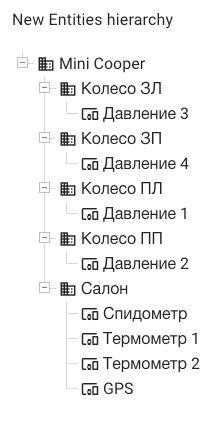
\includegraphics[scale=0.8]{pictures/5.jpg}
		\caption{Иерархия автомобиля}
		\label{fig1}
	\end{figure}
	\begin{chapter}{Основная часть}

\section{Постановка задачи}
	\begin{enumerate} 
      \item[1)]  Создание датчиков.
      \item[2)]  Генерация отправки данных на устройства.
      \item[3)] Анализ и обработка данных.
      \item[4)] Создание умных оповещений.
    \end{enumerate}

\section{Общая архитектура системы}

    Для создания проекта использовались платформа Thingsboard и графический конфигуратор для интернета вещей Node-red. Реализация работы выполнена и выложена в репозиторий на  \href{https://github.com/alexeyhorkin/IoT_UNN_HW}{github}, запуск осуществляется с  помошью docker.
    
    \textbf{Thingsboard} - платформа IoT с открытым исходным кодом, через которую происходило управление устройствами, сбор, обработка и визуализация данных.
    
    \textbf{Node-red} - графический конфигуратор, который позволяет через браузер построить схему взаимодействия устройст между собой и внешними системами.
    
\section{Node-Red}

    На изображении мы можем видеть четыре цепочки данных. С помощью них генерируются и отправляются данные о давлении, температурах, местоположении и скорости.
    
    \begin{figure}[!ht]
		\centering
		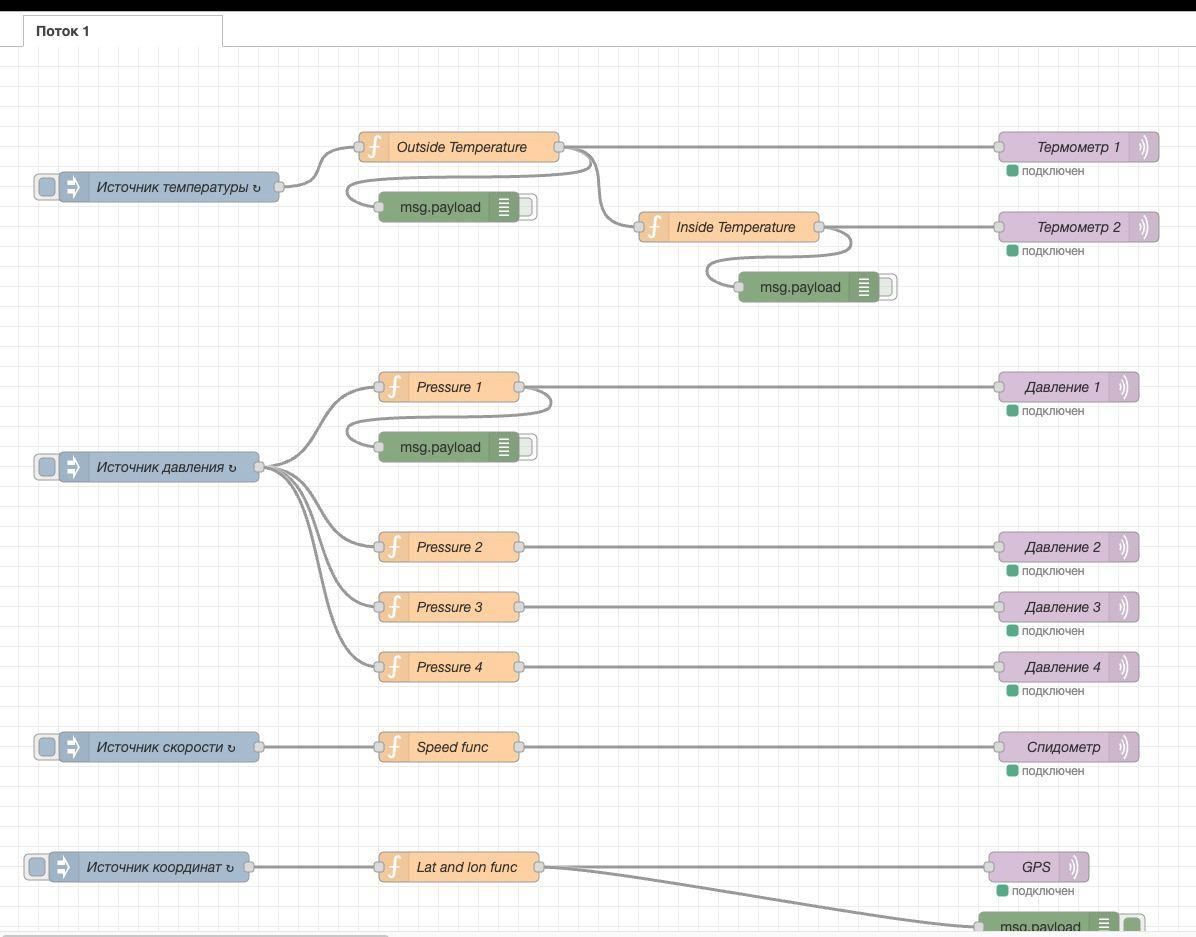
\includegraphics[scale=0.4]{pictures/8.jpg}
		\caption{Node-Red архитектура.}
		\label{fig1}
	\end{figure}
	

\section{Thingsboard}

    Для создания проекта нам потребовались следующие активы: <<Mini Cooper>>, <<Колесо ЗЛ>>, <<Колесо ЗП>>, <<Колесо ПЛ>>, <<Колесо ПП>>. В каждом из них указаны взаимоотношения между собой, при этом образуется иерархия.
    
    Были и созданы необходимые устройства: <<Давление 1-4>>, <<Температура 1-2>>, <<Спидометр>>, <<GPS>>.
    
    \begin{figure}[!ht]
		\centering
		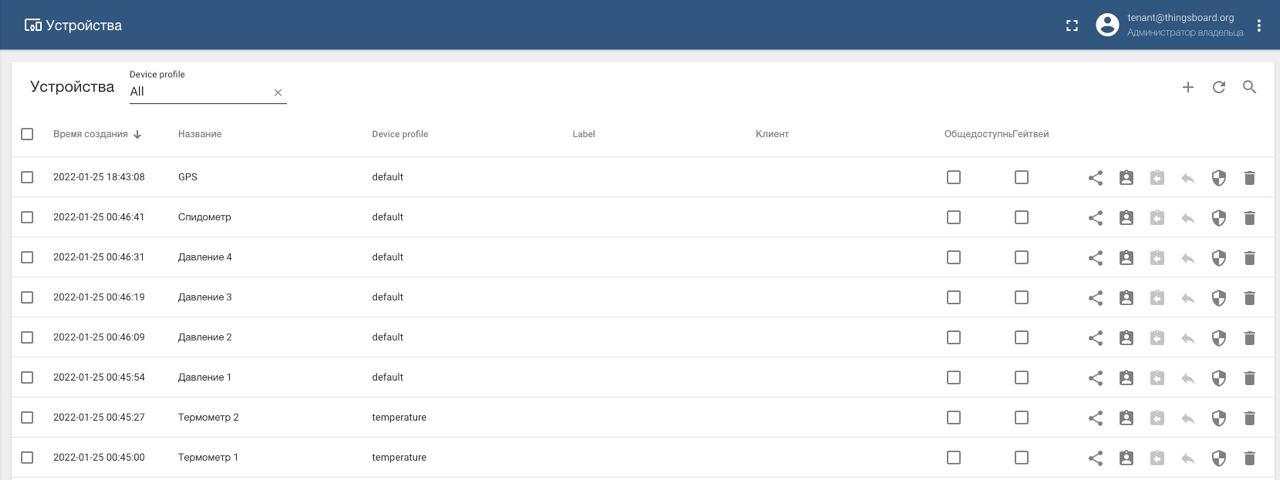
\includegraphics[scale=0.4]{pictures/4.jpg}
		\caption{Используемые устройства в Thingsboard.}
		\label{fig1}
	\end{figure}

    На главном экране дашборда располагаются виджеты:
    
	\begin{enumerate} 
      \item[1)]  Иерархия активов и устройств.
      \item[2)]  Карта с местоположением автомобиля.
      \item[3)]  Виджеты датчиков давления на каждое колесо.
      \item[4)]  Виджет спидометра.
      \item[5)]  Виджеты внутренней и внешней температур.
    \end{enumerate}

    \begin{figure}[!ht]
		\centering
		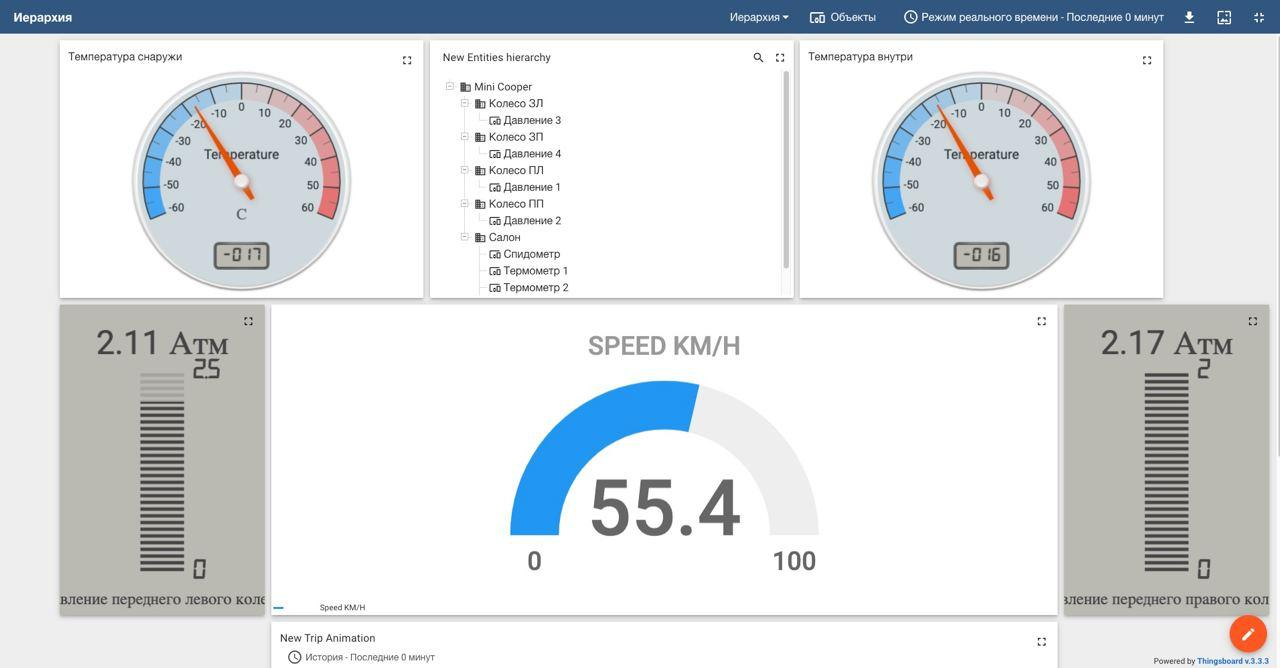
\includegraphics[scale=0.5]{pictures/2.jpg}
		\caption{Виджеты в Thingsboard.}
		\label{fig1}
	\end{figure}

    \begin{figure}[!ht]
		\centering
		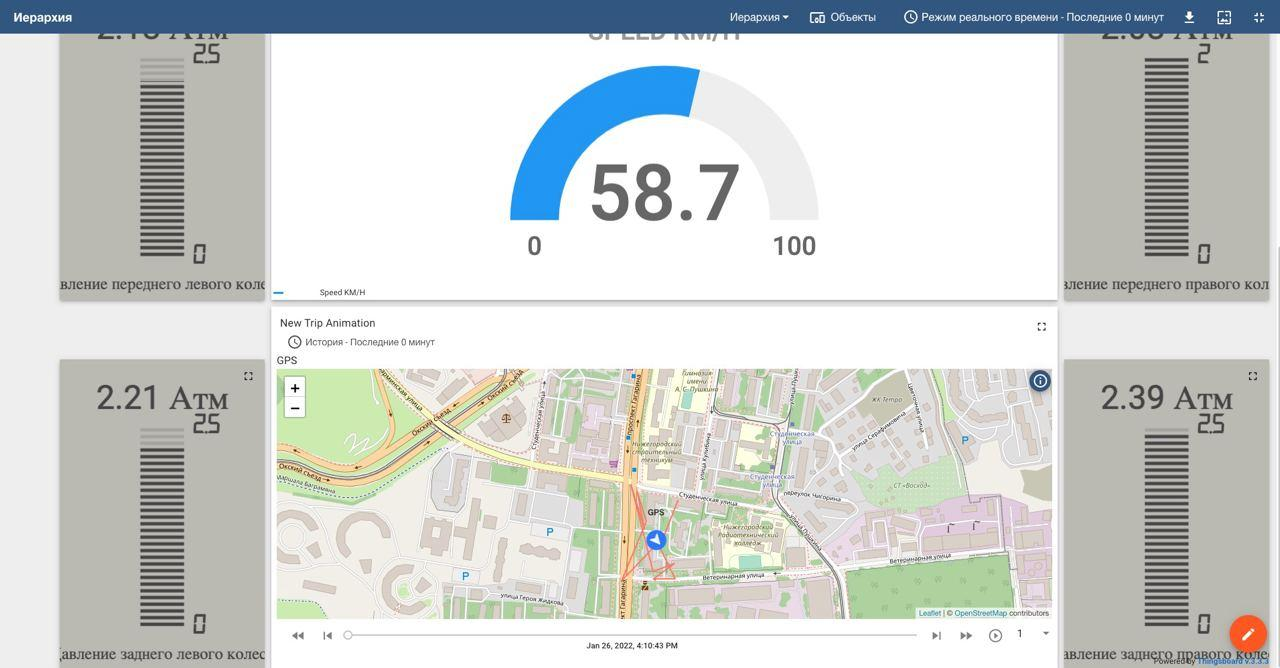
\includegraphics[scale=0.5]{pictures/3.jpg}
		\caption{Виджеты в Thingsboard.}
		\label{fig1}
	\end{figure}
	
В другом дашборде расположена информация о данных датчика внутренней температуры. Информация представлена в следующем виде:

	\begin{enumerate} 
      \item[1)]  График.
      \item[2)]  Оповещения.
    \end{enumerate}
    
    \begin{figure}[!ht]
		\centering
		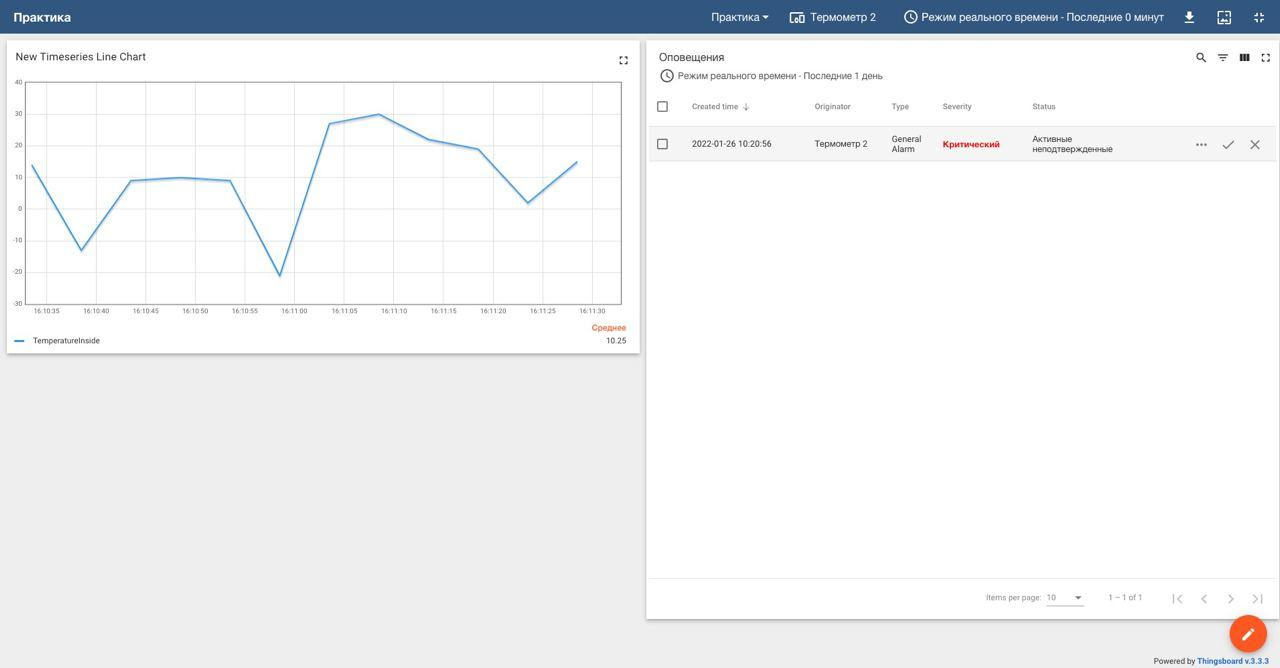
\includegraphics[scale=0.5]{pictures/1.jpg}
		\caption{Виджет графика внутренней температуры в Thingsboard.}
		\label{fig1}
	\end{figure}

Была реализована цепочка для работы датчиков.

\newpage

    \begin{figure}[!ht]
		\centering
		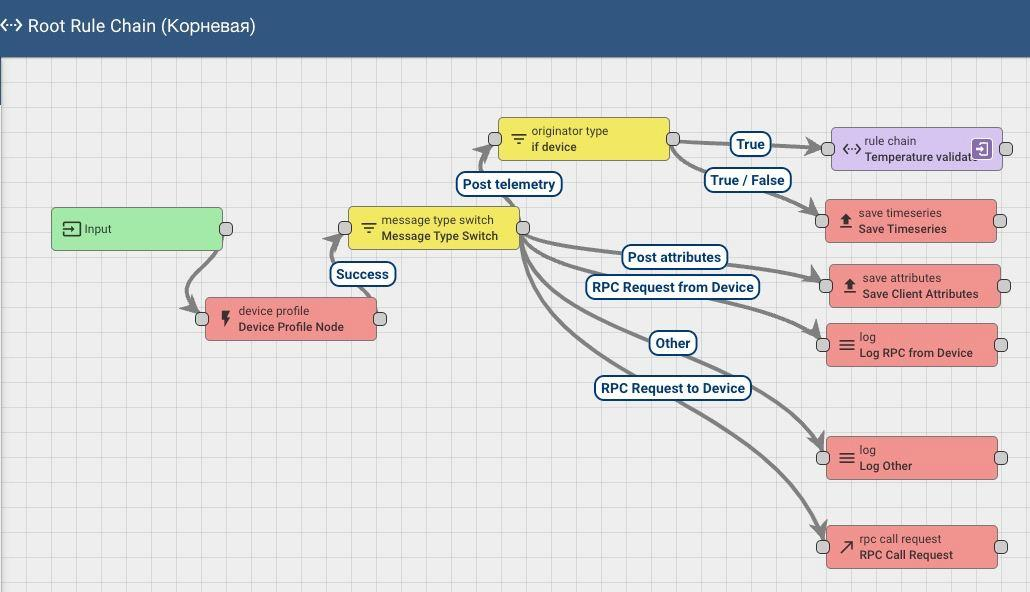
\includegraphics[scale=0.6]{pictures/6.jpg}
		\caption{Цепочка для работы датчиков.}
		\label{fig1}
	\end{figure}


В цепочке валидации температуры мы проверяем, что данные пришли с температурного сенсора, ответственного за температуру внутри салона. Затем, мы извлекаем серверные атрибуты <<maxTemp>> и <<minTemp>> с устройства, на основе которых происходит валидация. И в зависимости от результата создается определенное оповещение, сохраняется телеметрия, а также отправляется уведомление на почту.

    \begin{figure}[!ht]
		\centering
		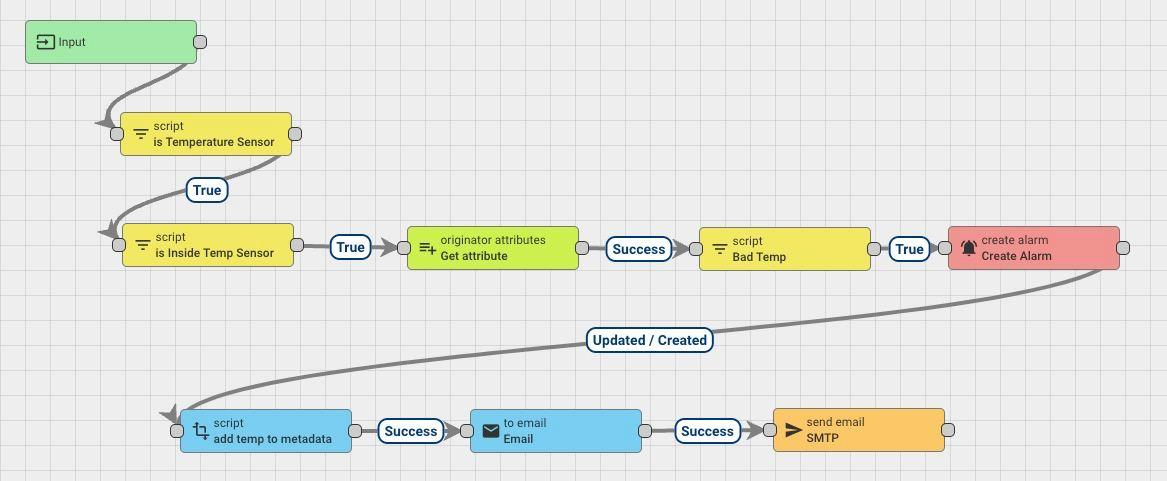
\includegraphics[scale=0.55]{pictures/7.jpg}
		\caption{Цепочка для работы предупреждений.}
		\label{fig1}
	\end{figure}

\newpage
\end{chapter}

	\likechapter{Заключение}

В ходе работы нами были изучены платформы: Thingsboard и инструмент разработки визуального программирования Node-red, с помощью которых был создан проект <<Mini Cooper 2.0>>, который получает, анализирует, обрабатывает данные и уведомляет о критических значениях данных с помощью сообщения на почту.

$$\\[7in]$$
Ссылка на репозиторий с проектом: https://github.com/alexeyhorkin/IoT\_UNN\_HW
	% \bibliography{bibliography}
	% \input{attachment}

\end{document}